\documentclass[14pt,fleqn]{extarticle}
\RequirePackage{prepwell-eng}

\previewoff 

\begin{document} 
\begin{problem}
	\statement 
    
    If the tangent to a curve at any point $P = (x,y)$ meets the coordinate
    axes at $A$ and $B$ such that $P$ is the mid-point of $AB$, then find the equation 
    of the curve given that it passes through $(1,1)$
    
    \begin{step}
  \begin{options} 
     \correct 
       
       In the figure below, $AB$ is some tangent, $A = (0,a), B = (b,0)$ and $P=(x,y)$ 
       
       \begin{center}
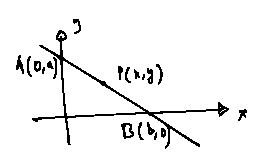
\includegraphics[scale=1.4]{1417-A.eps}
\end{center}

     \[\qquad \therefore \dydx = -\frac{a}{b} = -\frac{y}{x} \]
       
     \incorrect
     
     In the figure below, $AB$ is some tangent, $A = (0,a), B = (b,0)$ and $P=(x,y)$ 
       
       \begin{center}
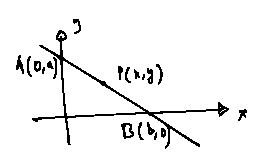
\includegraphics[scale=1.4]{1417-A.eps}
\end{center}

     \[\qquad \therefore \dydx = -\frac{a}{b} = -\frac{x}{y} \]
        
    \end{options} 
     \reason 
     
     If the tangent cuts the axes at $A$ and $B$ respectively and $P$ 
     is the mid-point, then 
     \[ \underbrace{P = \left(x,y \right) = \left(\frac{0+b}{2},\frac{0+a}{2} \right) = \left(\frac{b}{2}, \frac{a}{2} \right)}_{\text{Mid-point Rule}} \]
       
       Which means, 
       \begin{align}
       x = \frac{b}{2}&\text{ and } y = \frac{a}{2} \\
       \therefore b = 2x&\text{ and } a = 2y 
\end{align}

Moreover, the \underline{slope of the tangent} is 
\[ \quad \dydx = \dfrac{a-0}{0-b} = -\frac{a}{b} = -\frac{2y}{2x} = -\frac{y}{x}\]

Hence, the \underline{differential equation} for the curve
\[ \qquad\qquad \dydx = -\frac{y}{x}\]
\end{step}

\begin{step}
  \begin{options} 
     \correct 
       \[ \qquad\dydx = -\frac{y}{x}\implies xy = C \]
       And as the curve passes through $(1,1)$
       \[ \qquad C =1\text{ and } xy = 1\]
     \incorrect
     
       \[ \qquad\dydx = -\frac{y}{x}\implies y = e^x + C \]
       And as the curve passes through $(1,1)$
       \[ \qquad C = 1-e \text{ and } y = e^x + (1-e) \]
        
    \end{options} 
     \reason 
       
       \begin{align}
       \dydx = -\frac{y}{x} &\implies \frac{dy}{y} = -\frac{dx}{x} \\
       \therefore \int\frac{dy}{y} &= -\int\frac{dx}{x} \\
       \text{or } \log y &= -\log x + C_1 \\
       \implies \log y + \log x &= \log \left(xy \right) = C_1 \\
       \therefore xy &= e^{C_1} = C 
\end{align}

       But as the curve passes through $(1,1)$
       \[ \qquad\qquad C = 1\cdot 1 = 1\]
       And hence $\underbrace{xy = 1}_{C = 1}$
\end{step}
\end{problem} 
\end{document} 